\section{Discussion}


\subsection{Profile plots}


Figure \ref{fig:Profiles} shows the latitude profiles of the different models in differential flux. The flux increases towards the Galactic plane. Left-right assymmetry close to the Galactic center. 


\begin{figure*}[h!]
    \begin{subfigure}{0.5\textwidth}
        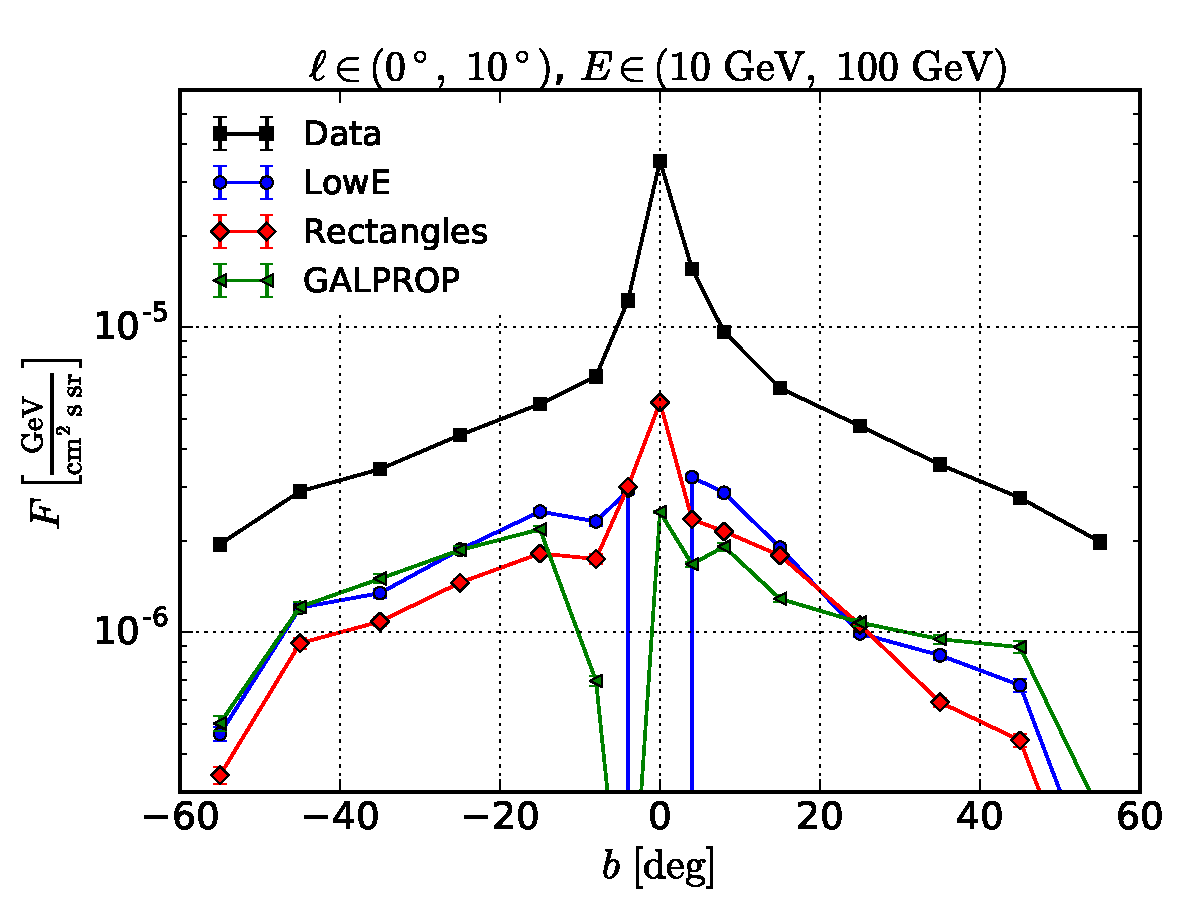
\includegraphics[width=\textwidth]{plots/Profiles_l=1_source_range_1.pdf}
    \end{subfigure} 
    \begin{subfigure}{0.5\textwidth}
        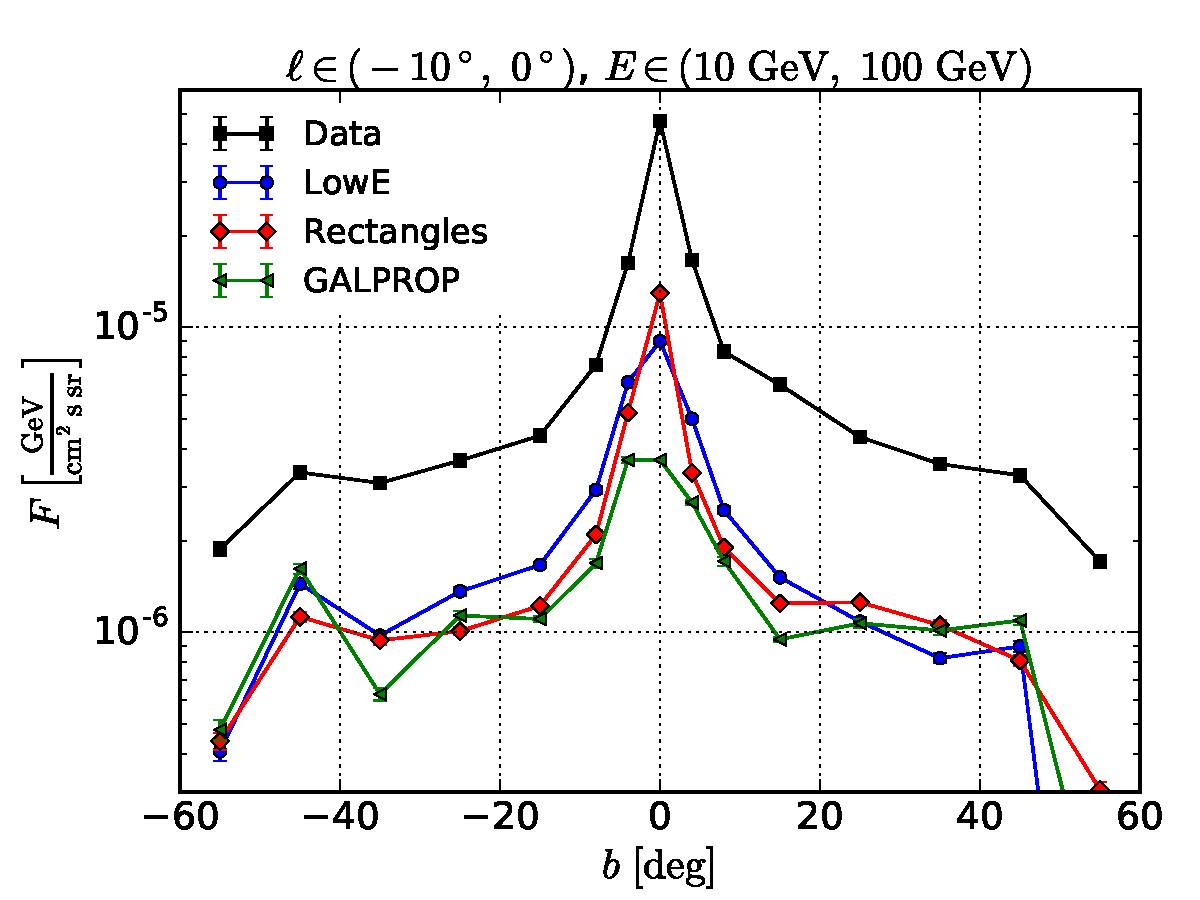
\includegraphics[width=\textwidth]{plots/Profiles_l=0_source_range_1.pdf}
    \end{subfigure}
  	\caption{Latitude profiles of the different models.}
  	\label{fig:Profiles}
\end{figure*}

\subsection{Comparison of the spectra at different latitudes}

Figure \ref{fig:SED_all} shows a comparison of the SED of the raw data (without point sources) and the three different models in a very thin latitude stripe covering the Galactic plane. The grey triangles show the difference in the raw data West minus East. All models give similar results. \\
\\
\begin{figure*}[h!]
    \begin{subfigure}{0.5\textwidth}
        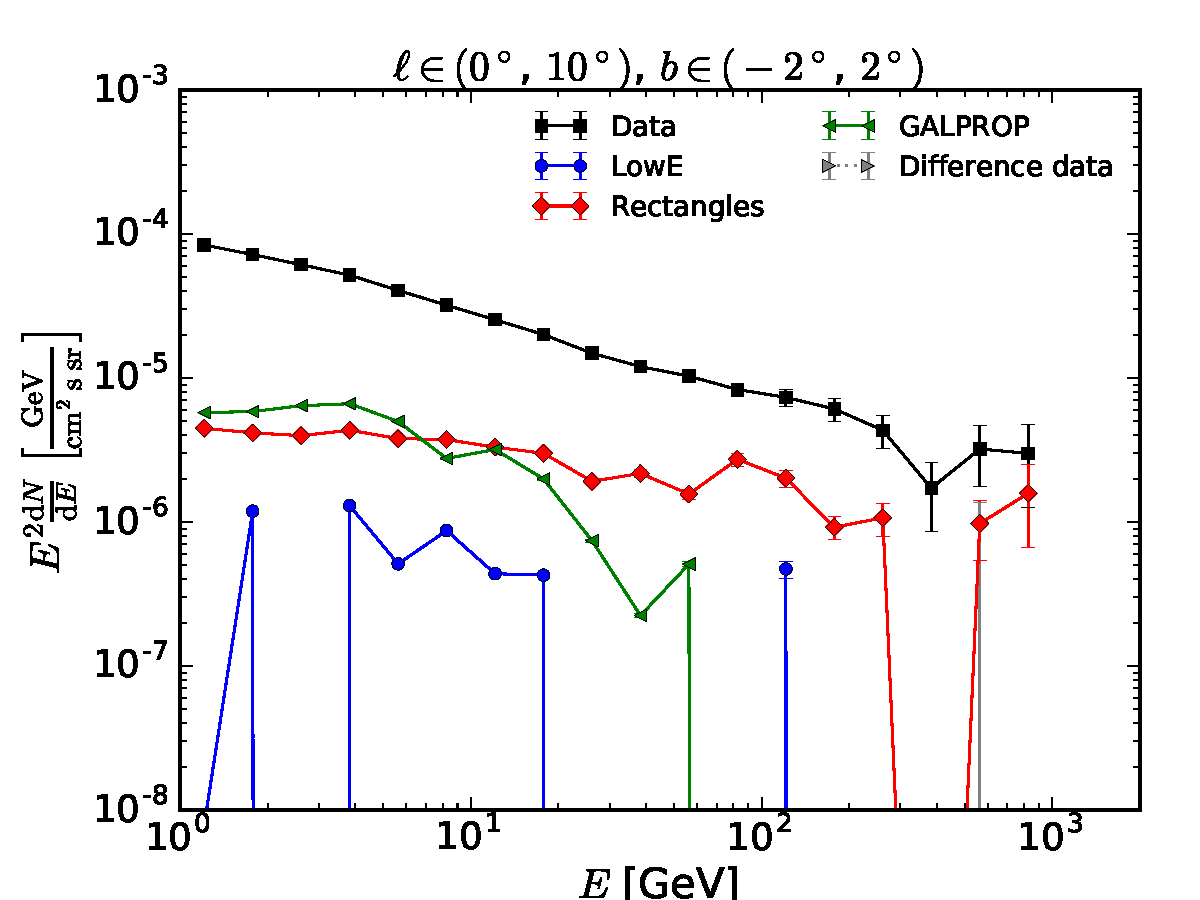
\includegraphics[width=\textwidth]{plots/SED_all_models_source_l=5_b=0.pdf}
    \end{subfigure} 
    \begin{subfigure}{0.5\textwidth}
        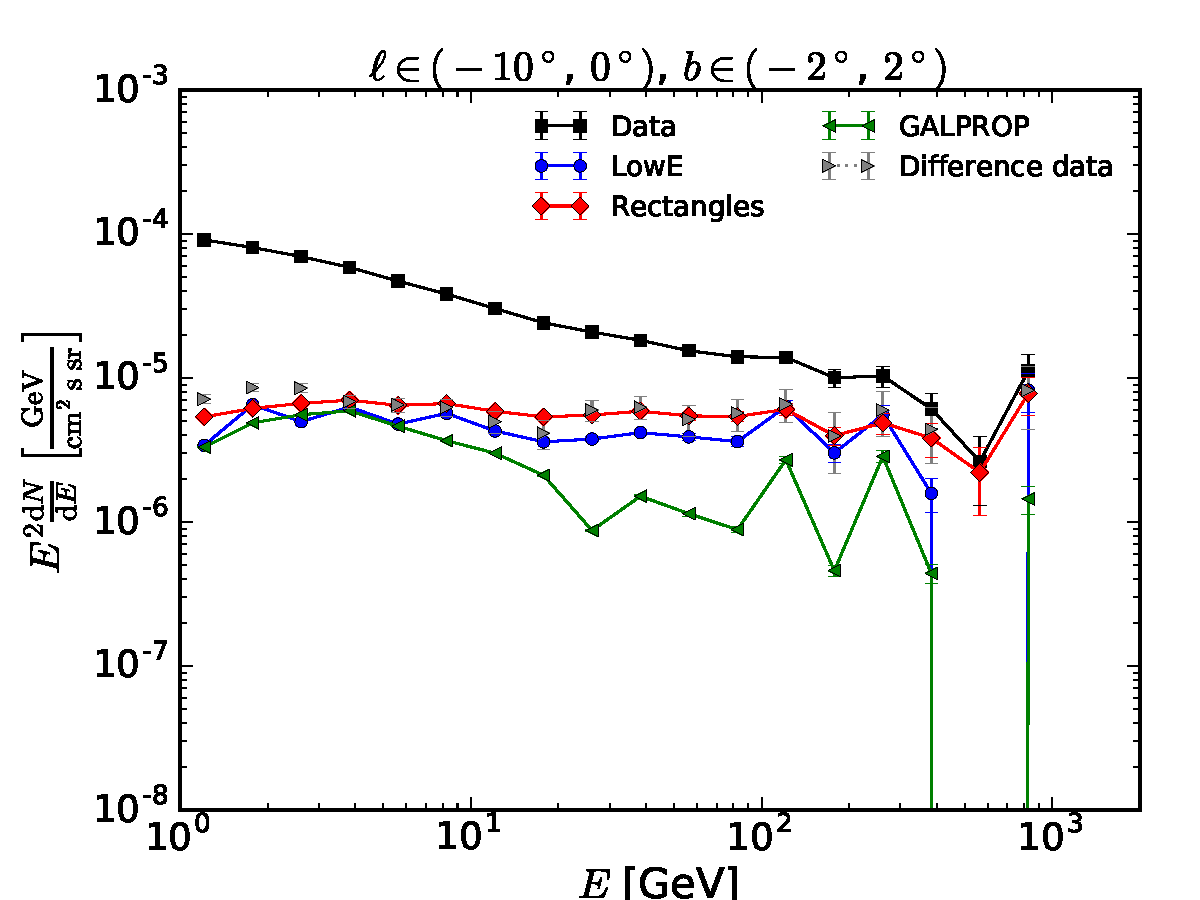
\includegraphics[width=\textwidth]{plots/SED_all_models_source_l=-5_b=0.pdf}
    \end{subfigure}
  	\caption{Comparison of SED of all models.}
  	\label{fig:SED_all}
\end{figure*}

To compare the behavior of the energy spectra at high energies for different latitudes, 
we fit a log-parabola
 \be
 f(E) = N_0 E^{-\alpha - \beta \ln(E)}
 \ee
in each latitude stripe. The local ``index'' of the spectrum at energy $E$ is
 \be 
n \equiv \frac{\de \ln f}{\de \ln E} = -\alpha - 2 \beta \ln(E).
 \ee
In Figure \ref{fig:logpar_index} we show a comparison of the SED index $(2 - n)$
for the bubbles spectra in different models at $E = 500$ GeV.
For positive longitudes the index is relatively soft ($n < -2$) for most of the latitudes, 
except high latitudes where the gamma-ray statistics is small.
For negative longitudes the index is near the GC is $\approx -2$, 
which is significantly harder than the index at higher latitudes.
\begin{figure*}[h!]
    \begin{subfigure}{0.5\textwidth}
        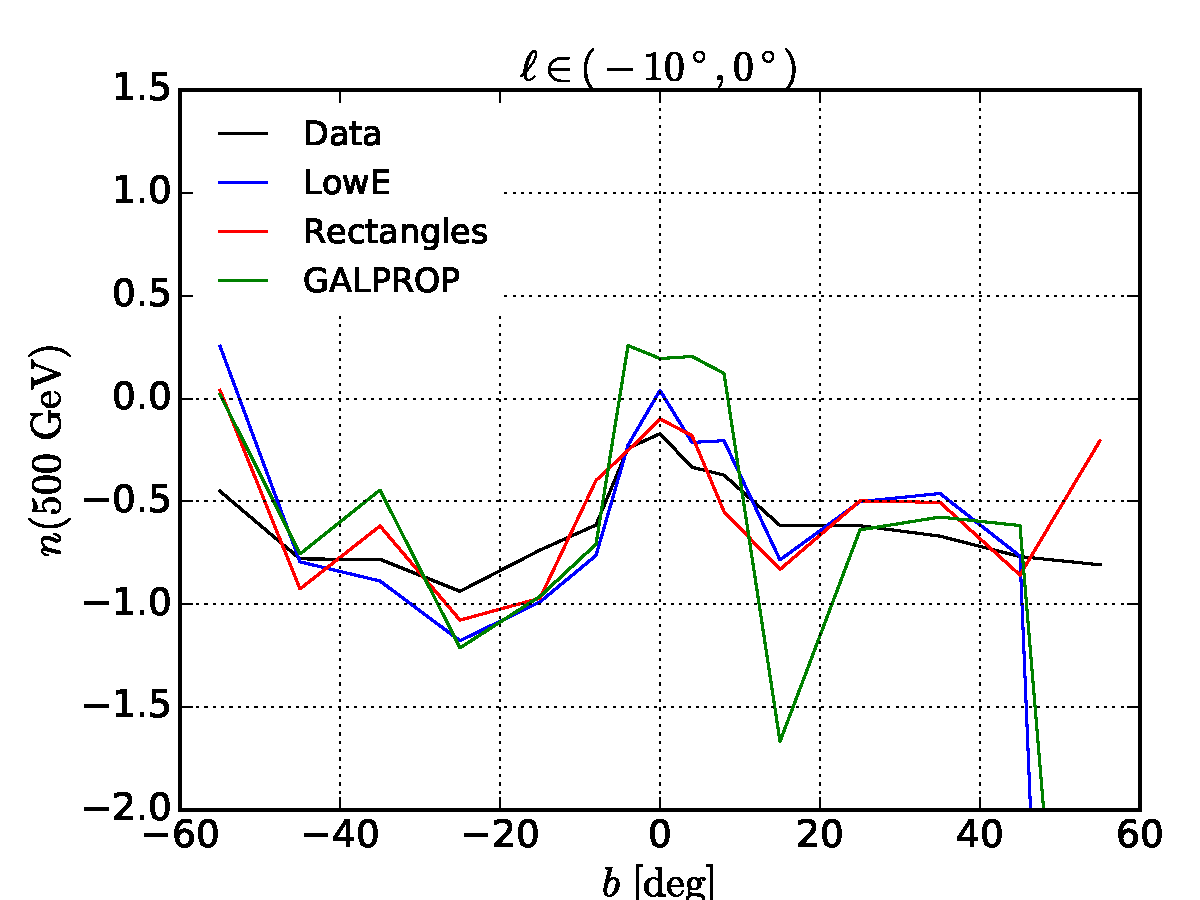
\includegraphics[width=\textwidth]{plots/LogParabola_n(500GeV)_l_in_(-10,0).pdf}
    \end{subfigure} 
    \begin{subfigure}{0.5\textwidth}
        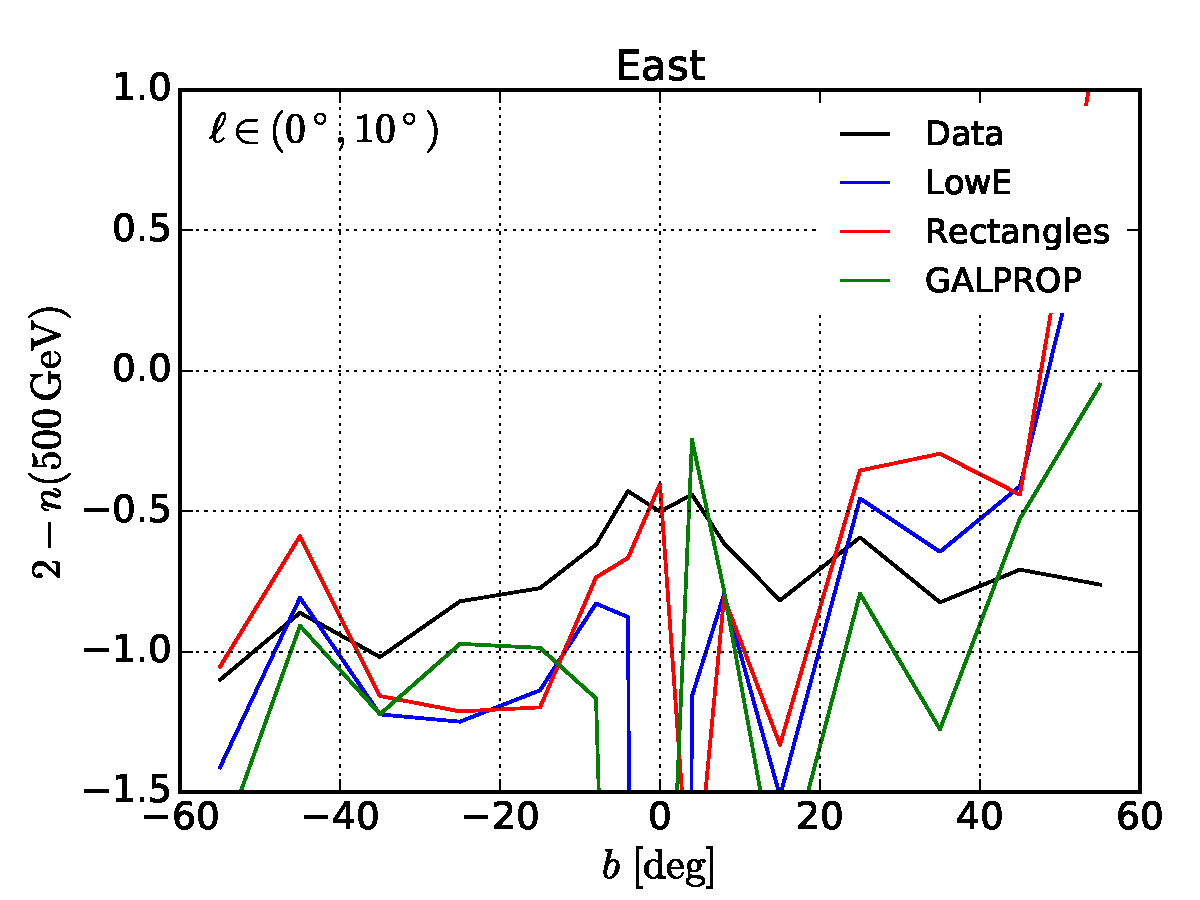
\includegraphics[width=\textwidth]{plots/LogParabola_n(500GeV)_l_in_(0,10).pdf}
    \end{subfigure}
  	\caption{``Index'' of the log-parabola at energy $E\ = \SI{500}{GeV}$.}
  	\label{fig:logpar_index}
\end{figure*}


\begin{figure*}[h!]
    \begin{subfigure}{0.5\textwidth}
        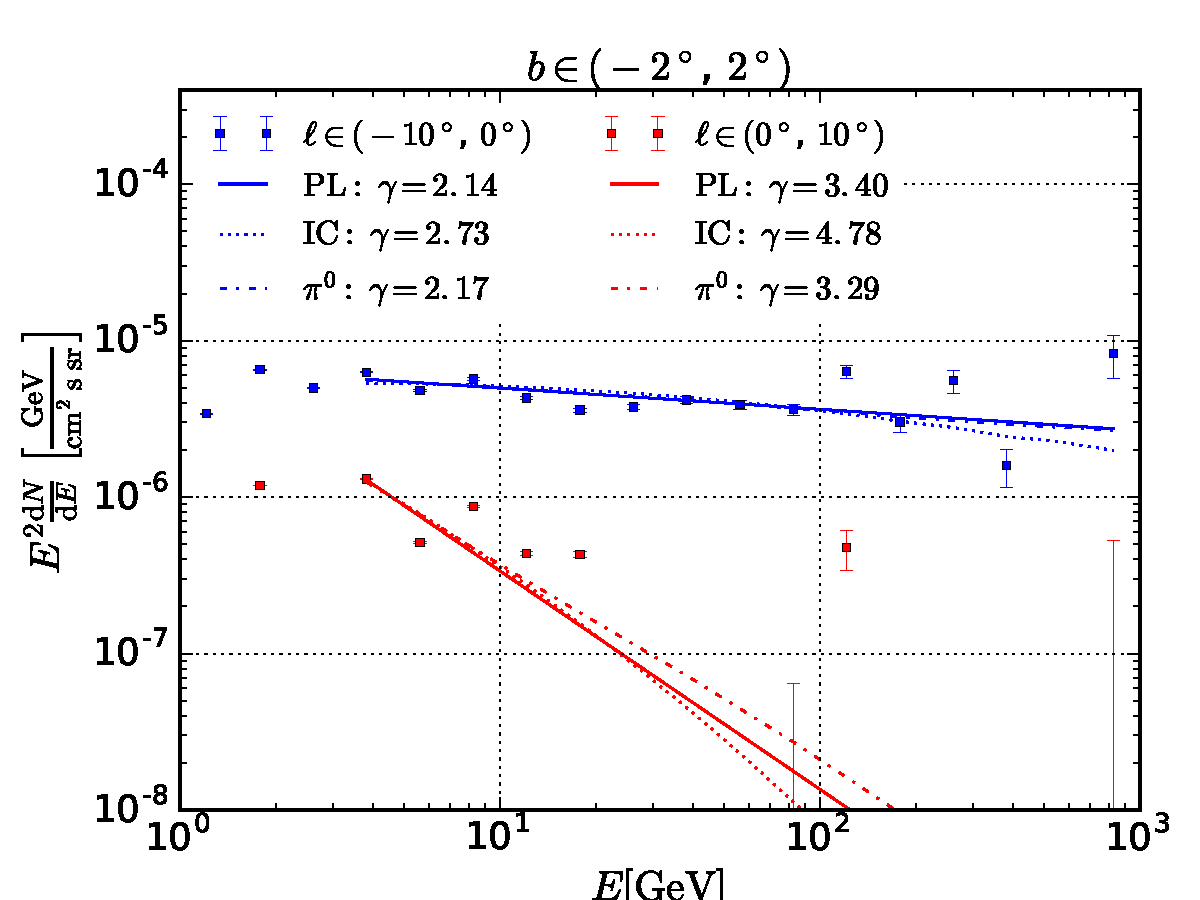
\includegraphics[width=\textwidth]{plots/SED_lowE_source_0.pdf}
    \end{subfigure} 
    \begin{subfigure}{0.5\textwidth}
        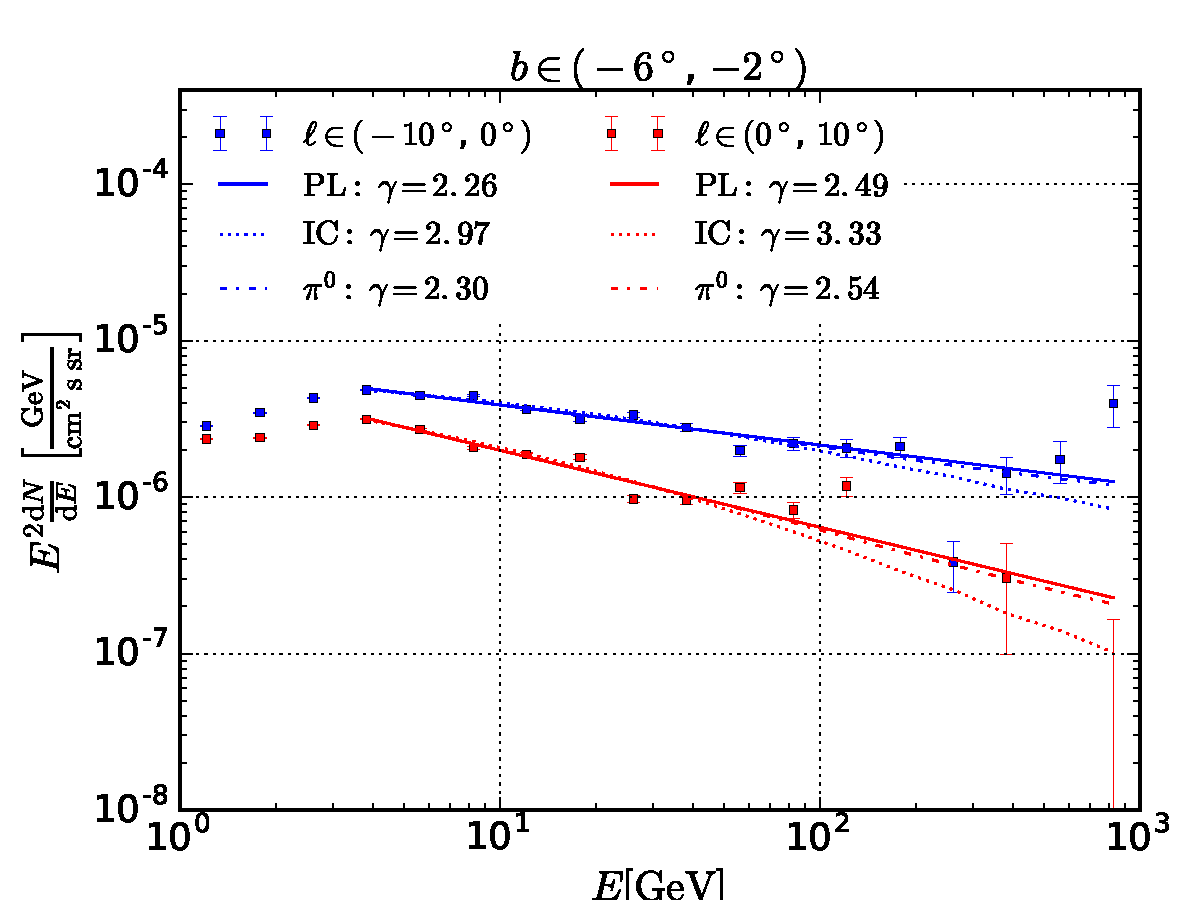
\includegraphics[width=\textwidth]{plots/SED_lowE_source_-4.pdf}
    \end{subfigure}
  	\caption{SED of low-energy model with powerlaw and particle spectra fits.}
  	\label{fig:SED_with_fits}
\end{figure*}




\subsection{IC model of the gamma-ray emission}
\label{sec:IC_model}

IC radiation is produced in scattering processes of relativistic electrons on photons of the ISRF. The spectrum of the IC gamma radiation $(E \de n/ \de E)_{\gamma,\IC}\ [\SI{}{1/cm^3s}]$ depends on the density of ISRF photons $(\de n/ \de E)_\ISRF [\SI{}{1/GeVcm^3}]$ , the density of electrons $(\de n / \de E)_\el\ [\SI{}{1/GeVcm^3}]$and the IC cross section $\sigma_\IC(E_\gamma, E_\ISRF, E_\el)$, taken from \citep{1970RvMP...42..237B}:
\be
\left(E\frac{\de n}{\de E}\right)_{\!\!\gamma,\IC}\! = c\int\!\! \int \left(\frac{\de n}{\de E}\right)_{\!\!\ISRF} \sigma_\IC\ \left(\frac{\de n}{\de E}\right)_{\!\!\el} \de E_\ISRF\, \de E_\el.
\label{eq:IC_spectrum}
\ee
The ISRF has three main components: starlight, IR and CMB. 
The IR and the starlight components are taken from the on-line distribution of GALPROP. 
For the CMB, we use the thermal spectrum with the temperature $\SI{2.73}{K}$. 
We assume that the distribution of electrons follows  a simple powerlaw
%\be 
%\left(\frac{\de n}{\de E}\right)_\el = n_\el \left(\frac{E}{\SI{1}{GeV}}\right)^{-\gamma_\el} \cdot \eto^\frac{E}{E_{\cut,\el}},
%\ee
and determine the normalization $n_\el$ and spectral index $\gamma_\el$  by fitting the IC spectrum\eqref{eq:IC_spectrum} to the diffuse \Fermi data using Poisson likelihood.  Point sources are masked as described in Section \ref{sec:data_diff}.\\
Figure \ref{fig:SED_with_fits} shows the residual spectrum in the low-energy model within the latitude stripes $b \in (-\ang{2}, \ang{2})$ and $b \in (-\ang{6}, -\ang{2})$. The dotted line represents the best-fit IC spectrum for an electron distribution following a simple powerlaw. \\
\\
For the latitude stripe covering the Galactic plane, $b \in (-\ang{2}, \ang{2})$, adding a cutoff to the powerlaw does not improve the $\chi^2$-value at negative longitudes (blue, $\chi^2 \approx 715$ in both cases) . For positive longitudes both a simple powerlaw and a powerlaw with a cutoff have similarly high $\chi^2$-values due to the large oversubtractions. For negative longitudes we find a lower bound for the cutoff energy at $\SI{14.9}{TeV}$, for positive longitudes at $\SI{16.1}{GeV}$, at a $\SI{95}{\percent}$-confidence level.\\
\\
Slightly below the Galactic plane, $b \in (-\ang{6}, -\ang{2})$, the $\chi^2$-value does not improve by adding a powerlaw, neither at negative longitudes ($\chi^2 = 99$ in both cases) nor at positive longitudes ($\chi^2 = 155$ in both cases). For negative longitudes we find a lower bound for the cutoff energy at $\SI{22.0}{TeV}$, for positive longitudes at $\SI{790.0}{GeV}$, at a $\SI{95}{\percent}$-confidence level.\\
\\

\dima{ we should first show here the fit with a simple power law (no cutoff) and then find the difference in $\chi^2$
for the models with and without the cutoff.
In the model with a cutoff, we should use the errors on the cutoff to determine 95\% lower confidence limit on the cutoff value.}








\subsection{Hadronic model of gamma-ray emission}
\label{sec:Pion_model}

In the hadronic model, the gamma rays are produced as a result of collisions of hadronic CR with the interstellar gas.
The spectrum of the gamma radiation $(E \de n / \de E)_{\gamma,\pi^0}\ [\SI{}{1/cm^3s}]$ depends on the density of interstellar gas, where we assume $n_\Hy = \SI{1}{/cm^3}$, the velocity of CR protons, which we approximate with the speed of light, $v_\pr \approx c$, the energy density of CR protons $(\de n / \de T)_\pr\ [\SI{}{1/GeVcm^3}]$ and the cross section to produce gamma rays in a proton-nucleus collisions $\sigma_\pr (E_\gamma, T_\pr)$, \Laura{which Dima saved in numpy arrays}:
\be
\left(E\frac{\de n}{\de E}\right)_{\!\!\gamma, \pi^0}\! = \int n_\Hy\ \sigma_\pr v_\pr \left(\frac{\de n}{\de T}\right)_{\!\!\pr} \de T_\pr,
\ee
where the integral goes over the kinetic energies of the protons $T_\pr$. 